
% Gemini theme
% https://github.com/anishathalye/gemini

\documentclass[final]{beamer}

% ====================
% Packages
% ====================

\usepackage[T1]{fontenc}
\usepackage{lmodern}
\usepackage[size=custom,width=120,height=72,scale=1.0]{beamerposter}
\usetheme{gemini}
\usecolortheme{mit}
\usepackage{graphicx}
\usepackage{booktabs}
\usepackage{tikz}
\usepackage{pgfplots}
\pgfplotsset{compat=1.14}
\usepackage{anyfontsize}
\usepackage{dsfont}
\usepackage{fontawesome5}

% ====================
% Lengths
% ====================

% If you have N columns, choose \sepwidth and \colwidth such that
% (N+1)*\sepwidth + N*\colwidth = \paperwidth
\newlength{\sepwidth}
\newlength{\colwidth}
\setlength{\sepwidth}{0.025\paperwidth}
\setlength{\colwidth}{0.3\paperwidth}

\newcommand{\separatorcolumn}{\begin{column}{\sepwidth}\end{column}}

% ====================
% Title
% ====================

\title{How well-behaved are revisions to quarterly fiscal data in the euro area?}

\author{Krzysztof Bankowski \inst{1} \and Thomas Faria \inst{2} \and Robert Schall \inst{3}}

\institute[shortinst]{\inst{1} European Central Bank \samelineand \inst{2} Insee \samelineand \inst{3} European University Institute}

% ====================
% Footer (optional)
% ====================
 
\footercontent{
  \href{https://thomasfaria.github.io/Quarterly_GFS_revisions/}{\faIcon{github} \url{https://thomasfaria.github.io/Quarterly_GFS_revisions/}} 
  \hfill
  NTTS Conference 2023, Brussels
  }
% (can be left out to remove footer)

% ====================
% Logo (optional)
% ====================

% use this to include logos on the left and/or right side of the header:
\logoright{
  
\includegraphics{Logo_Insee.png}
  \hspace*{0.75cm}
  
\includegraphics{Logo_European_Central_Bank_resized.png}}
\logoleft{\includegraphics[width=0.3\linewidth]{QRCODE.pdf}}

% ====================
% Body
% ====================

\begin{document}

\begin{frame}[t]
\begin{columns}[t]
\separatorcolumn

\begin{column}{\colwidth}
 
  \begin{alertblock}{Summary}
    \textbf{Objective:}
    \begin{itemize}
      \item Determine how well-behaved fiscal revisions are, especially by contrasting them with macro revisions.
    \end{itemize}

    \textbf{Results:}
    \begin{itemize}
      \item Creation a real-time fiscal quarterly dataset for the euro area countries.
      \item We derive a broad set of statistics that allow us to assess the properties of the revisions.
      \item Fiscal revisions, like macro revisions, DO NOT satisfy desirable properties expected from well-behaved revisions.
      \item When contrasted with macro revisions, fiscal revisions are quite comparable (most notably after 2014).
    \end{itemize}

  \end{alertblock}

  \begin{block}{Motivation}

    \begin{itemize}
      \item Most macroeconomic data are subject to \textbf{revisions}.
      \item Researchers and policy-makers have no choice rather than \textbf{recognising and understanding} data revisions.
      \item \textbf{Often heard view} is that fiscal revisions are particularly bad.
      \item Well-behaved revisions ought to carry certain \textbf{characteristics}, according to the relevant literature:
      \begin{itemize}
        \item zero bias
        \item little dispersion 
        \item no predictability in real time
      \end{itemize}
      \item (Our study is a comprehensive analysis of revisions to \textbf{quarterly fiscal data in the euro area}.)
    \end{itemize}
  \end{block}

  \begin{block}{Definitions}
    \begin{itemize}
      \item \textbf{Final revision} for a quarter $t$: $r_t^f =. x_t^f - x_t^1$
      \item Final value $x_t^f$ and we define it as October T+1 release.
      \item \textbf{Intermediate revisions} $r_t^i = x_t^{i+1} - x_t^i$ make up for final revisions.
      \item All revisions are based on \textbf{annual growth differences}.
      \item Our dataset relies on quarterly \textbf{GFS} supplemented with \textbf{MNA}.
  \end{itemize}

  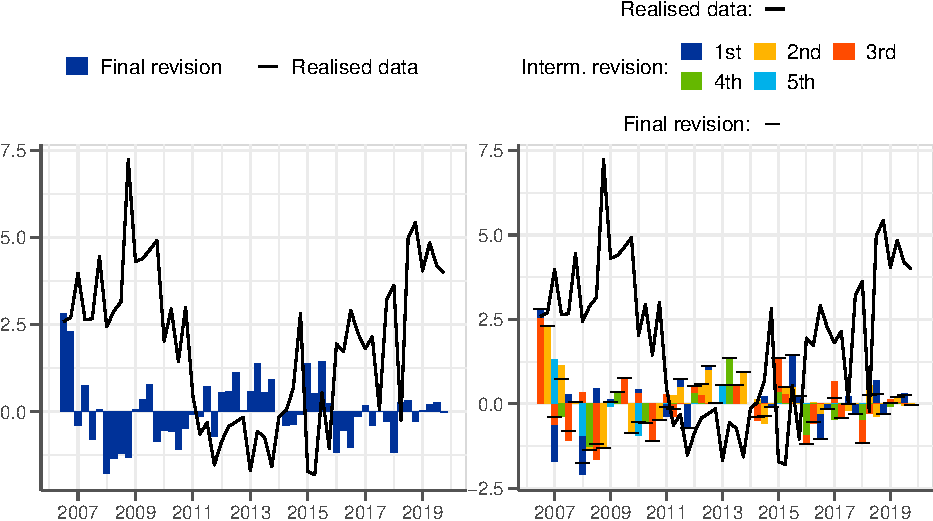
\includegraphics[width=1\linewidth]{poster-plots_files/figure-pdf/fig-dataoverview1-1.pdf} 

  \end{block}
\end{column}

\separatorcolumn

\begin{column}{\colwidth}

  \begin{block}{Real-time quarterly fiscal dataset}
    \begin{itemize}
      \item Our dataset relies on quarterly \textbf{GFS} (Government Finance Statistics) supplemented with \textbf{MNA} (Main National Accounts).
      \item It includes 15 \textit{fiscal} series and 6 \textit{macroeconomic} series. 
      \item Our dataset consists of 65 quarterly vintages taking place since January 2007 to February 2023. We restricted our analysis to pre-covid period (i.e. final values for 2019).
      \item We are committed to open science and have made both the dataset and the replicatory files are \textbf{open source}. Scan the QR code to access them!
    \end{itemize}

    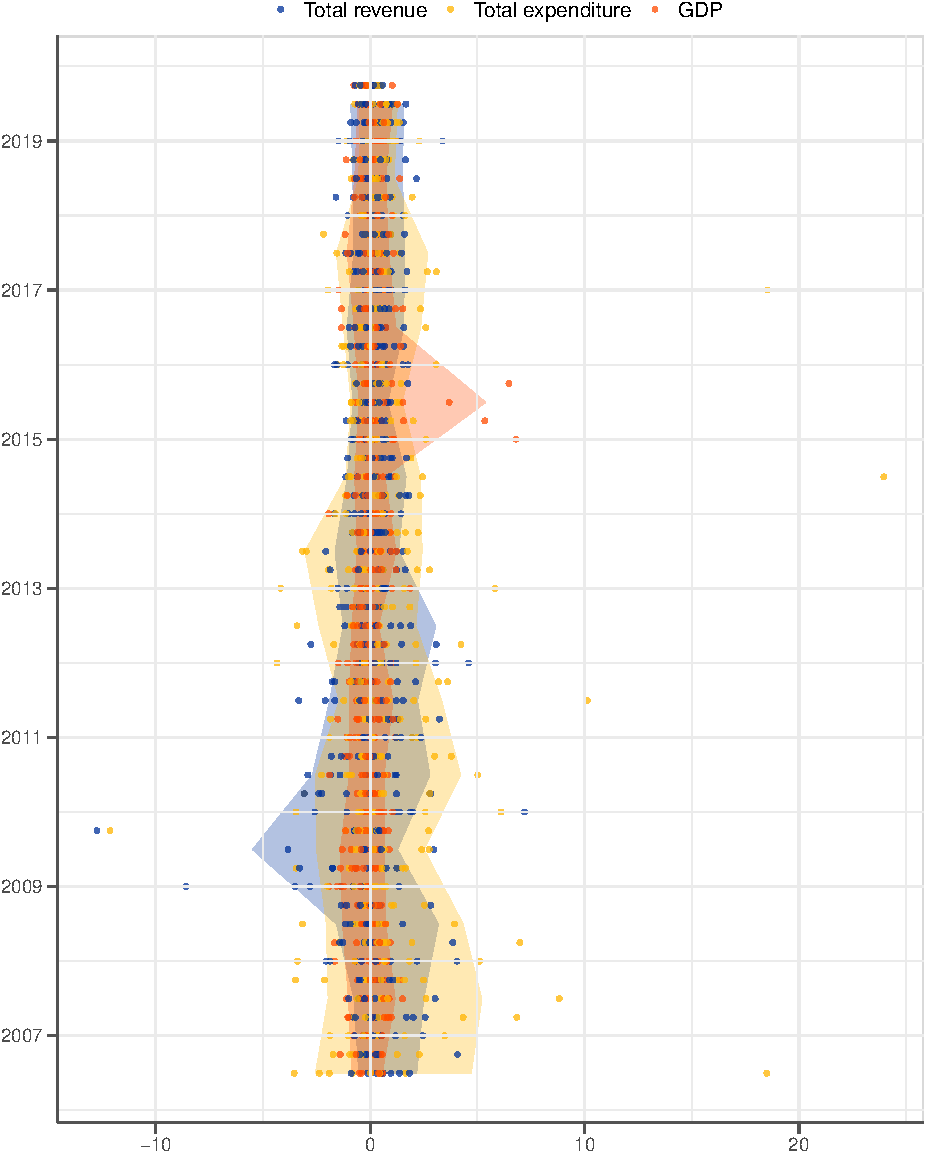
\includegraphics[width=1\linewidth]{poster-plots_files/figure-pdf/fig-revisions_over_time-1.pdf} 


  \end{block}

  \begin{block}{Unconditional properties of revisions}
    \includegraphics[width=1\linewidth]{poster-plots_files/figure-pdf/fig-RevGItems_post2014-1.pdf} 

    \begin{itemize}
      \item We look at a set of summary statistics including the mean revision (\textbf{MR}), the maximum and the minimum revision (\textbf{MAX} and \textbf{MIN}), the mean absolute revision (\textbf{MAR}), the root-mean-square revision (\textbf{RMSR}) and, finally, the noise-to-signal ratio (\textbf{N2S}).
      \item Almost all variables we consider in the analysis are associated with a \textbf{positive bias}, as judged by the MR statistic. \item Other measures, namely MIN-MAX range, MAR and RMSR, indicate that the revisions tend to have \textbf{large dispersion}.
      \item The degree of \textit{misbehaviour} of fiscal revisions \textit{after 2014} is comparable to \textit{macroeconomic} series revisions.
    \end{itemize}

  \end{block}

\end{column}
\separatorcolumn


\begin{column}{\colwidth}



  \begin{block}{Forecastability of revisions}

    \textbf{Key question}: is the complete model better than the naive model? In other words, does any information available at the time of the initial release have predictive power?

    \textbf{Naive model}: 
    \[
    r_{t,m}^{f} = \epsilon_{t,m}
    \]
    %\bigskip{}
    \textbf{Complete model}: 
    \[
      r_{t,m}^{f} = \sum_{m=1}^{9}\beta_{m}C_{m} 
    + \sum_{j=1}^{4} \gamma_{j}Q_{t}^{j} 
    + \omega\mathds{1}_{\left[t\geq2014Q2\right]}
    + \delta x_{t,m}^{1} 
    + \sum_{i=1}^{S} \rho_{i}\left(x_{t-i,m}^{i+1}-x_{t-i,m}^{1}\right)
    + \epsilon_{t,m}
    \]

    \begin{tabular}{lll}
         $C_{m}$ & $\rightarrow$ & country dummies \\
         $Q_{t}^{j}$ & $\rightarrow$ & quarter dummies \\
         $\mathds{1}_{\left[t\geq2014Q2\right]}$ & $\rightarrow$ & ESA 2010 introduction dummy \\
         $x_{t,m}^{1}$ & $\rightarrow$ & initial release \\
         $\left(x_{t-i,m}^{i+1}-x_{t-i,m}^{1}\right)$ & $\rightarrow$ & past revisions \\
      \end{tabular}

    \vspace*{0.5cm}

    There are two equally effective methods for assessing predictive power: examining the \textbf{RMSE reduction} or conducting the \textbf{joint F-test}.

    \vspace*{0.5cm}
    \textbf{Result}:
    \begin{itemize}
      \item Irrespective of fiscal and macro variables, we found a model that outperforms the naive model, indicating the existence of \textbf{predictability} in real-time revisions. Specifically, we identified that the initial release holds significant predictive power for subsequent revisions.
    \end{itemize} 

  \end{block}

  \begin{block}{Intermediate revisions}

    \begin{itemize}
      \item Intermediate revisions do not provide additional information about the unconditional properties of revisions compared to final revisions.
      \item Fiscal series undergo more significant revisions during EDP notifications (April and October), whereas macro series are subject to continuous revisions regardless of the quarter
    \end{itemize} 

    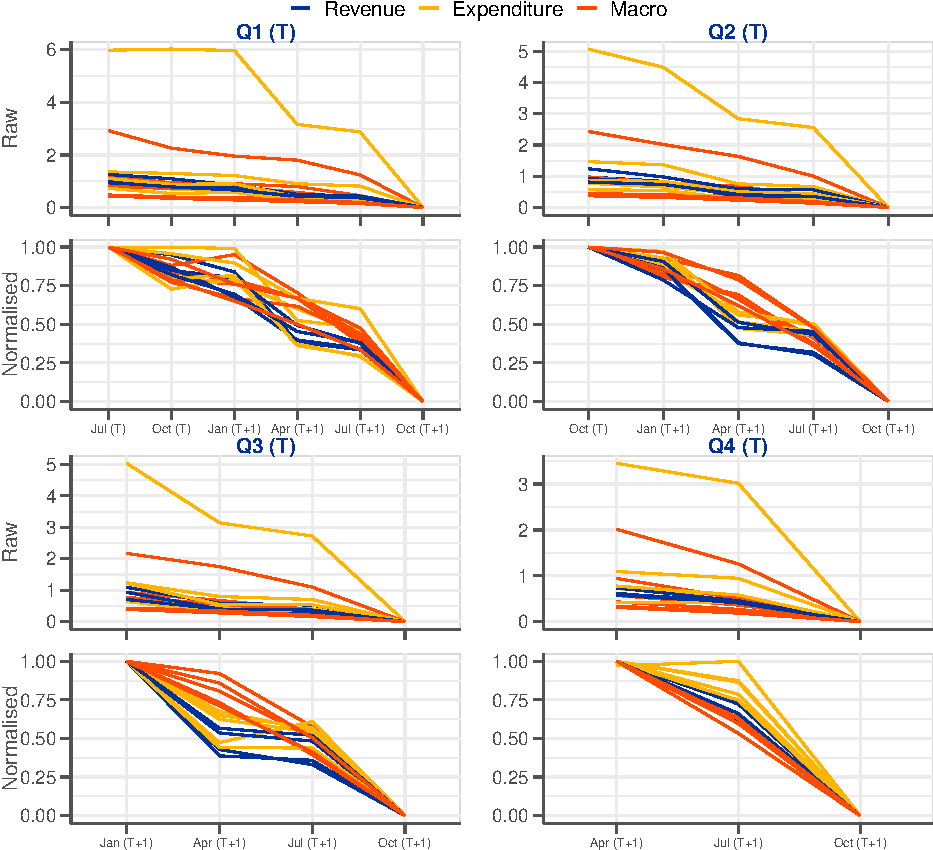
\includegraphics[width=1\linewidth]{poster-plots_files/figure-pdf/fig-Single_Rev_Path-1.pdf} 

  \end{block}

  \begin{block}{Selected literature}
    \nocite{*}
    \footnotesize{\bibliographystyle{plain}\bibliography{poster}}

  \end{block}

\end{column}

\separatorcolumn
\end{columns}
\end{frame}

\end{document}

